\documentclass{beamer}
\setbeamertemplate{navigation symbols}{}
\usetheme{Warsaw}
\xdefinecolor{darkgreen}{rgb}{0,0.35,0}
\usecolortheme[named=darkgreen]{structure}
\beamersetuncovermixins{\opaqueness<1>{25}}{\opaqueness<2->{15}}
\usepackage{graphicx}

\begin{document}
\title{Software Testing the Numpy Linear Algebra Library}  
\author{Group 7}

\date{\today} 
\begin{frame}
\titlepage
\end{frame}

\begin{frame}\frametitle{Table of contents}\tableofcontents
\end{frame} 

\section{Library Choice}
\begin{frame}
\frametitle{Library Choice} 
\begin{itemize}
\item Sufficiently large\\
\item Contains at least one "complicated" function\\
\item Reasonable inputs \\
\end{itemize}
\end{frame}

%\begin{frame}\frametitle{Table of contents}\tableofcontents
%\end{frame}
\begin{frame}\frametitle{Considered Libraries} 
\begin{itemize}
\item Reinforcement Learning Library - Complicated input 
\item Numpy sorting - Too small (?)
\item Numpy logical - no "complicated" functions 
\item Numpy Linalg
\end{itemize}
\end{frame}


\begin{frame}\frametitle{Numpy Linear Algebra Library} 
\begin{itemize}

\item functions for matrix or vector operations 
\item 30 functions
\item take matrix/vector inputs
\end{itemize}
\end{frame}

\section{Black Box Testing}
\begin{frame}\frametitle{Black Box Testing} 
Goal:Derive a set of input cases that fully exercise the external functionality\\

-As we are not dealing with the structure of the program we mostly focus on the information i.e. inputs and outputs
\end{frame}

\begin{frame}\frametitle{Identifying flaws} 
\begin{itemize}
\item Problems with usability
\item Performace problems
\item Input parameter cases
\end{itemize}
\end{frame}

\begin{frame}\frametitle{Numpy Documentation} 
	See Numpy Documentation of the Linear Algebra library.
\end{frame}


\begin{frame}\frametitle{Black Box Testing} 
Plan to black-box test as many functions as possible\\
Test to see if the inputs/outputs match what is given in the documentation
\begin{itemize}
\item Standard inputs
\item Edge cases
\item Exceptions 
\end{itemize}
\end{frame}

\begin{frame}\frametitle{Black Box Testing: Example numpy.linalg.dot()} 
Testing the basic properties of a dot product 
\begin{itemize}
	\item $ a \bullet b = b \bullet a $
	\item $ a \bullet (\textbf{r}b + c) = \textbf{r}(a \bullet b) + (a \bullet c) $
	\\
	\item $ a \bullet 0 = 0 $
	\item $ a \bullet a = | a^2 |$
\end{itemize}
\end{frame}



\begin{frame}\frametitle{Black Box Testing: Raising Exception} 
Since it is not possible to multiply to matrices if their last dimension are not the same.
\begin{figure}[h]
	\centering
	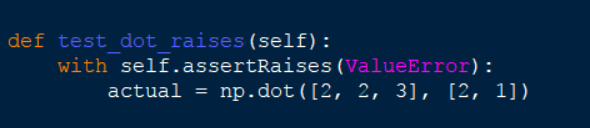
\includegraphics[width=0.70\textwidth]{images/raises.png}
	\caption{Raising exception in dot product.}
	\label{fig:rai}
\end{figure}
\end{frame}


\section{White-Box}
\begin{frame}\frametitle{White-Box testing} 
\begin{itemize}
\item Test for edge coverage using Coverage.py
 notes which parts of the code have been executed, and analyzes the source to identify code that could have been executed but was not.
\item Need to create a collection of test inputs that cause all edges to execute
\item Still need to choose which function
\end{itemize}
\end{frame}

\begin{frame}\frametitle{Numpy's Tests}
\begin{itemize}
	\item Numpy’s own tests
	\\ Test functions for linalg module”, 1700 rows. 
	\\ class LinalgCase(object):
	\\ don’t test raw data, they first build test objects containing 4 objects. 
	\\ self.name; self.a; self.b; self.tags  
\end{itemize}
\end{frame}

\begin{frame}\frametitle{Numpy's Tests}
\begin{itemize}
\item 3 main types of cases (tags): square or non-square, Hermitian
\item square:
\\CASES = []
\\ CASES +=  LinalgCase("single", array([[1., 2.], [3., 4.]], dtype=single), array([2., 1.], dtype=single)),
\\ CASES +=   LinalgCase("cdouble", array([[1. + 2j, 2 + 3j], [3 + 4j, 4 + 5j]], dtype=cdouble), array([2. + 1j, 1. + 2j], dtype=cdouble)),
\\ CASES +=  LinalgCase("8x8", np.random.rand(8, 8), np.random.rand(8)),
\\  0x0, 1x1, "nonarray", "matrixOnly", "2matrices", 
\end{itemize}
\end{frame}

\begin{frame}\frametitle{Numpy's Tests}
\begin{itemize}
\item non-square: 
\\ CASES += LinalgCase("single\_nsq\_1", array([[1., 2., 3.], [3., 4., 6.]], dtype=single),array([2., 1.], dtype=single)),
\item Hermitian: 
\\CASES += LinalgCase("hsingle", array([[1., 2.], [2., 1.]], dtype=single), None),
\item Combine the 3 above types into generic object
\\def \_make\_generalized\_cases():
\item Get all combination of all cases – Cartesian product. 
\\def \_make\_strided\_cases(): #stride combination 
\item Now the testing part starts:
\item class LinalgSquareTestCase(object):
\\def test\_sq\_cases(self):
	\end{itemize}
\end{frame}




\begin{frame}
Any Questions?
\end{frame}


\end{document}